\documentclass{ximera}

%\usepackage{todonotes}

\newcommand{\todo}{}

\usepackage{tkz-euclide}
\tikzset{>=stealth} %% cool arrow head
\tikzset{shorten <>/.style={ shorten >=#1, shorten <=#1 } } %% allows shorter vectors

\usepackage{tkz-tab}  %% sign charts
\usetikzlibrary{decorations.pathreplacing} 

\usetikzlibrary{backgrounds} %% for boxes around graphs
\usetikzlibrary{shapes,positioning}  %% Clouds and stars
\usetikzlibrary{matrix} %% for matrix
\usepgfplotslibrary{polar} %% for polar plots
\usetkzobj{all}
\usepackage[makeroom]{cancel} %% for strike outs
%\usepackage{mathtools} %% for pretty underbrace % Breaks Ximera
\usepackage{multicol}

\usepackage{polynom}



\usepackage[many]{tcolorbox}  %% for titled boxes
\newtcolorbox{xbox}[1]{%
    tikznode boxed title,
    enhanced,
    arc=0mm,
    interior style={white},
    attach boxed title to top center= {yshift=-\tcboxedtitleheight/2},
    fonttitle=\bfseries,
    colbacktitle=white,coltitle=black,
    boxed title style={size=normal,colframe=white,boxrule=0pt},
    title={#1}}


\usepackage{array}
\setlength{\extrarowheight}{+.1cm}   
\newdimen\digitwidth
\settowidth\digitwidth{9}
\def\divrule#1#2{
\noalign{\moveright#1\digitwidth
\vbox{\hrule width#2\digitwidth}}}





\newcommand{\RR}{\mathbb R}
\newcommand{\R}{\mathbb R}
\newcommand{\N}{\mathbb N}
\newcommand{\Z}{\mathbb Z}

%\renewcommand{\d}{\,d\!}
\renewcommand{\d}{\mathop{}\!d}
\newcommand{\dd}[2][]{\frac{\d #1}{\d #2}}
\newcommand{\pp}[2][]{\frac{\partial #1}{\partial #2}}
\renewcommand{\l}{\ell}
\newcommand{\ddx}{\frac{d}{\d x}}
\newcommand{\ddt}{\frac{d}{\d t}}

\newcommand{\zeroOverZero}{\ensuremath{\boldsymbol{\tfrac{0}{0}}}}
\newcommand{\inftyOverInfty}{\ensuremath{\boldsymbol{\tfrac{\infty}{\infty}}}}
\newcommand{\zeroOverInfty}{\ensuremath{\boldsymbol{\tfrac{0}{\infty}}}}
\newcommand{\zeroTimesInfty}{\ensuremath{\small\boldsymbol{0\cdot \infty}}}
\newcommand{\inftyMinusInfty}{\ensuremath{\small\boldsymbol{\infty - \infty}}}
\newcommand{\oneToInfty}{\ensuremath{\boldsymbol{1^\infty}}}
\newcommand{\zeroToZero}{\ensuremath{\boldsymbol{0^0}}}
\newcommand{\inftyToZero}{\ensuremath{\boldsymbol{\infty^0}}}



\newcommand{\numOverZero}{\ensuremath{\boldsymbol{\tfrac{\#}{0}}}}
\newcommand{\dfn}{\textbf}
%\newcommand{\unit}{\,\mathrm}
\newcommand{\unit}{\mathop{}\!\mathrm}
\newcommand{\eval}[1]{\bigg[ #1 \bigg]}
\newcommand{\seq}[1]{\left( #1 \right)}
\renewcommand{\epsilon}{\varepsilon}
\renewcommand{\iff}{\Leftrightarrow}

\DeclareMathOperator{\arccot}{arccot}
\DeclareMathOperator{\arcsec}{arcsec}
\DeclareMathOperator{\arccsc}{arccsc}
\DeclareMathOperator{\si}{Si}
\DeclareMathOperator{\proj}{proj}
\DeclareMathOperator{\scal}{scal}


\newcommand{\tightoverset}[2]{% for arrow vec
  \mathop{#2}\limits^{\vbox to -.5ex{\kern-0.75ex\hbox{$#1$}\vss}}}
\newcommand{\arrowvec}[1]{\tightoverset{\scriptstyle\rightharpoonup}{#1}}
\renewcommand{\vec}{\mathbf}
\newcommand{\veci}{\vec{i}}
\newcommand{\vecj}{\vec{j}}
\newcommand{\veck}{\vec{k}}
\newcommand{\vecl}{\boldsymbol{\l}}

\newcommand{\dotp}{\bullet}
\newcommand{\cross}{\boldsymbol\times}
\newcommand{\grad}{\boldsymbol\nabla}
\newcommand{\divergence}{\grad\dotp}
\newcommand{\curl}{\grad\cross}
%\DeclareMathOperator{\divergence}{divergence}
%\DeclareMathOperator{\curl}[1]{\grad\cross #1}


\colorlet{textColor}{black} 
\colorlet{background}{white}
\colorlet{penColor}{blue!50!black} % Color of a curve in a plot
\colorlet{penColor2}{red!50!black}% Color of a curve in a plot
\colorlet{penColor3}{red!50!blue} % Color of a curve in a plot
\colorlet{penColor4}{green!50!black} % Color of a curve in a plot
\colorlet{penColor5}{orange!80!black} % Color of a curve in a plot
\colorlet{fill1}{penColor!20} % Color of fill in a plot
\colorlet{fill2}{penColor2!20} % Color of fill in a plot
\colorlet{fillp}{fill1} % Color of positive area
\colorlet{filln}{penColor2!20} % Color of negative area
\colorlet{fill3}{penColor3!20} % Fill
\colorlet{fill4}{penColor4!20} % Fill
\colorlet{fill5}{penColor5!20} % Fill
\colorlet{gridColor}{gray!50} % Color of grid in a plot

\newcommand{\surfaceColor}{violet}
\newcommand{\surfaceColorTwo}{redyellow}
\newcommand{\sliceColor}{greenyellow}




\pgfmathdeclarefunction{gauss}{2}{% gives gaussian
  \pgfmathparse{1/(#2*sqrt(2*pi))*exp(-((x-#1)^2)/(2*#2^2))}%
}


%%%%%%%%%%%%%
%% Vectors
%%%%%%%%%%%%%

%% Simple horiz vectors
\renewcommand{\vector}[1]{\left\langle #1\right\rangle}


%% %% Complex Horiz Vectors with angle brackets
%% \makeatletter
%% \renewcommand{\vector}[2][ , ]{\left\langle%
%%   \def\nextitem{\def\nextitem{#1}}%
%%   \@for \el:=#2\do{\nextitem\el}\right\rangle%
%% }
%% \makeatother

%% %% Vertical Vectors
%% \def\vector#1{\begin{bmatrix}\vecListA#1,,\end{bmatrix}}
%% \def\vecListA#1,{\if,#1,\else #1\cr \expandafter \vecListA \fi}

%%%%%%%%%%%%%
%% End of vectors
%%%%%%%%%%%%%

%\newcommand{\fullwidth}{}
%\newcommand{\normalwidth}{}



%% makes a snazzy t-chart for evaluating functions
%\newenvironment{tchart}{\rowcolors{2}{}{background!90!textColor}\array}{\endarray}

%%This is to help with formatting on future title pages.
\newenvironment{sectionOutcomes}{}{} 



%% Flowchart stuff
%\tikzstyle{startstop} = [rectangle, rounded corners, minimum width=3cm, minimum height=1cm,text centered, draw=black]
%\tikzstyle{question} = [rectangle, minimum width=3cm, minimum height=1cm, text centered, draw=black]
%\tikzstyle{decision} = [trapezium, trapezium left angle=70, trapezium right angle=110, minimum width=3cm, minimum height=1cm, text centered, draw=black]
%\tikzstyle{question} = [rectangle, rounded corners, minimum width=3cm, minimum height=1cm,text centered, draw=black]
%\tikzstyle{process} = [rectangle, minimum width=3cm, minimum height=1cm, text centered, draw=black]
%\tikzstyle{decision} = [trapezium, trapezium left angle=70, trapezium right angle=110, minimum width=3cm, minimum height=1cm, text centered, draw=black]


\outcome{Identify word problems as related rates problems.}
\outcome{Solve related rates word problems.}
\outcome{Translate word problems into mathematical expressions.}

\title[Dig-In:]{Applied related rates}

\begin{document}
	\begin{abstract}
		We solve related rates problems in context.
	\end{abstract}
	\maketitle
	
	Now we are ready to solve related rates problems in context. Just as
	before, we are going to follow essentially the same plan of attack in
	each problem.
	
	
	\begin{description}
		\item[\textbf{Introduce variables, identify the given rate and the unknown rate.}] Assign a variable to each quantity that changes in time.
		\item[\textbf{Draw a picture.}] If possible, draw a schematic picture with all the relevant information. 
		\item[\textbf{Find equations.}] Write equations that relate all
		relevant variables.
		\item[\textbf{Differentiate with respect to t.}] Here we will often use
		implicit differentiation and obtain an equation that relates the given rate and the unknown rate. 
		\item[\textbf{Evaluate and solve.}] Evaluate
		each quantity at the relevant instant and solve for the unknown rate.
		
	\end{description}
	
	
	
	
	\section{Formulas}
	In our next problem, we will stretch and flatten a cylinder-shaped pizza dough.
	\begin{image}
		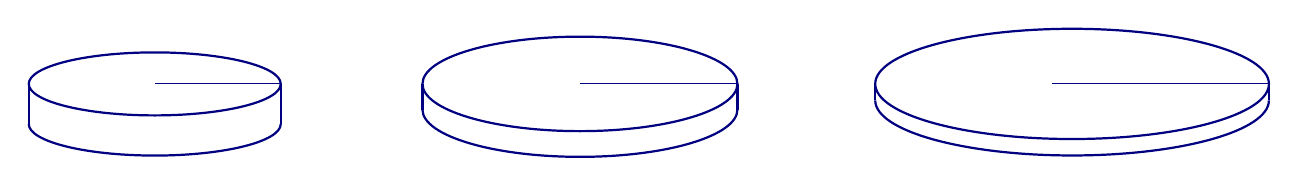
\begin{tikzpicture}
		\draw[penColor, thick] (-11.4,0) ellipse (1.6 and .4);
		\draw[ thick,penColor] (-13,-.51) arc (180:360:1.6 and .4);% bottom
		\draw[penColor] (-11.4,0) -- (-9.8,0);
		\draw[penColor, thick] (-13,0) -- (-13,-.51);
		\draw[penColor, thick] (-9.8,0) -- (-9.8,-.51);
		\draw[penColor, thick] (-6,0) ellipse (2 and .6);
		\draw[ thick,penColor] (-8,-.3264) arc (180:360:2 and .6);% bottom
		\draw[penColor] (-6,0) -- (-4,0);
		\draw[penColor, thick] (-4,0) -- (-4,-.3264);
		\draw[penColor, thick] (-8,0) -- (-8,-.3264);
		
		\draw[penColor, thick] (0.25,0) ellipse (2.5 and .7);
		\draw[ thick,penColor] (-2.25,-.208896) arc (180:360:2.5 and .7);% bottom
		\draw[penColor] (0,0) -- (2.75,0);
		\draw[penColor, thick] (-2.25,0) -- (-2.25,-.208896);
		\draw[penColor, thick] (2.75,0) -- (2.75,-.208896);
		
		
		
		\end{tikzpicture}
	\end{image}
	\begin{example}
		A hand-tossed pizza crust starts off as a ball of dough with a volume
		of $400\pi\, \text{cm}^3$. First, the cook stretches the dough to the
		shape of a cylinder of radius $12$ cm. Next the cook tosses the
		dough.
		
		If during tossing, the dough maintains the shape of a cylinder and the
		radius is increasing at a rate of $15$ cm/min, how fast is its
		thickness changing when the radius is $20$ cm?
		\begin{explanation}
			First, we \textbf{introduce the variables} $V$, $r$, and $h$, denoting the volume, the radius, and the thickness of the pizza, in that order. We \textbf{identify} the given rate $\frac{dr}{dt}=15$ cm/min and the unknown rate $\frac{dh}{dt}$, when $r=20$.   
			
			Next, we \textbf{draw a picture}. Note that our pizza dough is shaped as a cylinder.
			
			\begin{image}
				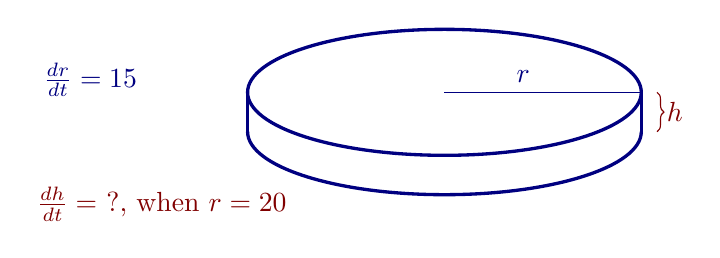
\begin{tikzpicture}
				\draw[penColor,very thick] (-0,0) ellipse (2.5 and .8);
				\draw[very thick,penColor] (-2.5,-.5) arc (180:360:2.5 and .8);% bottom
				\draw[penColor] (0,0) -- (2.5,0);
				\draw[penColor,very thick] (-2.5,0) -- (-2.5,-.5);
				\draw[penColor,very thick] (2.5,0) -- (2.5,-.5);
				\node[above,penColor] at (1,0) {$r$};
				\node[below,penColor] at (-4.5,0.5) {$\frac{dr}{dt} = 15$};
				\draw[penColor2,decoration={brace,raise=.2cm},decorate,thin] (2.5,0)--(2.5,-.5);
				\node [penColor2,right] at (2.7,-.25) {$h$};
				\node [penColor2, right] at (-5.3,-1.42) {$\frac{dh}{dt}=$ ?, when $r=20$};
				\end{tikzpicture}
			\end{image}
			Next we need to \textbf{find equations}. Recall the formula for the volume of the cylinder, $V=\pi\cdot r^2\cdot h$ and note that $V=400\pi\, \text{cm}^3$, and write
			\[
			400\pi = \pi \cdot r^2 \cdot h,
			\]
			which immediately simplifies to
			\[
			400 = r^2 \cdot h.
			\]
			Since both $r$ and $h$ are functions of time, we now  \textbf{differentiate} both sides of  the equation using implicit differentiation,
			
			\[
			0 = 2\cdot r \cdot \frac{dr}{dt} \cdot h+ r^2 \cdot \frac{dh}{dt}.
			\]
			Now we'll \textbf{evaluate} all  the quantities at the instant when $r=20$. 
			But, first, we have to compute $h$ at that moment. Since
			\[
			400 = 20^2 \cdot h ,
			\] it follows that $h=1$, when $r=20$. Now, we are ready to \textbf{solve}.
			
			\[
			0 = 2\cdot 20 \cdot 15 \cdot 1 + 20^2 \cdot \frac{dh}{dt}
			\]
			\[
			\frac{-2\cdot 20 \cdot 15 \cdot 1}{20^2} =  \frac{dh}{dt}
			\]
			Therefore, when $r=20$,
			
			\[
			\frac{dh}{dt} = -1.5.
			\]
			Hence, the thickness of the dough is changing at a rate of $\answer[given]{-1.5}$
			cm/min when $r=20$ cm.
		\end{explanation}
	\end{example}
	In our next example  we consider a melting snowball.
	\begin{image}
		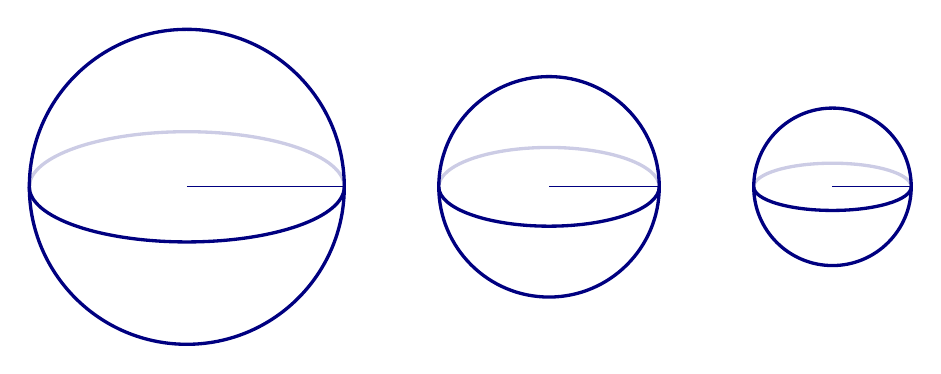
\begin{tikzpicture}
		%\draw[penColor!50!background,very thick] (0,0) ellipse (2 and 1);
		\draw[very thick,penColor!20!background] (-4,0) arc (0:180:2 and .7);% top half of ellipse
		\draw [penColor, very thick] (-6,0) circle [radius=2];
		\draw[penColor] (-6,0) -- (-4,0);
		
		\draw[very thick,penColor] (-2.8,0) arc (180:360:1.4 and .5);% bottom half of ellipse
		\draw[very thick,penColor!20!background] (0,0) arc (0:180:1.4 and .5);% top half of ellipse
		\draw [penColor, very thick] (-1.4,0) circle [radius=1.4];
		\draw[penColor] (-1.4,0) -- (0,0);
		
		\draw[very thick,penColor] (-8,0) arc (180:360:2 and .7);% bottom half of ellipse
		
		\draw[very thick,penColor] (1.2,0) arc (180:360:1 and .3);% bottom half of ellipse
		\draw[very thick,penColor!20!background] (3.2,0) arc (0:180:1 and .3);% top half of ellipse
		\draw [penColor, very thick] (2.2,0) circle [radius=1];
		\draw[penColor] (2.2,0) -- (3.2,0);
		\end{tikzpicture}
	\end{image}
	\begin{example}
		Consider a melting snowball. We will assume that the rate at which the
		snowball is melting is proportional to its surface area. Show that
		the radius of the snowball is changing at a constant rate.
		
		\begin{explanation}
			First, we \textbf{introduce the variables} $V$, $r$, and $A$, denoting the volume, the radius, and the surface area of the snowball, in that order . Then, we \textbf{identify} the given rate $\frac{dV}{dt}$  and the unknown rate $\frac{dr}{dt}$, the rate to be determined. This problem is a bit unusual, because``the given  rate" is not explicitly given. We will deal with this issue below. 
			Next, we \textbf{draw a picture}.
			\begin{image}
				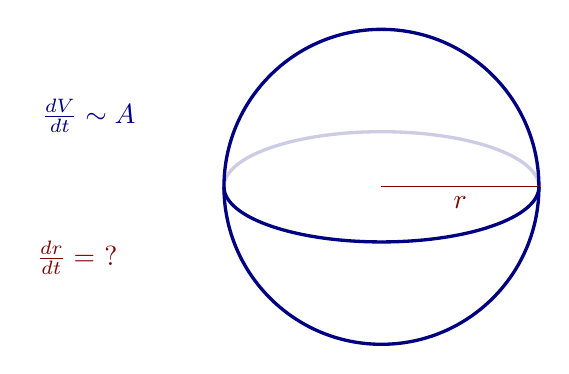
\begin{tikzpicture}
				%\draw[penColor!50!background,very thick] (0,0) ellipse (2 and 1);
				\draw[very thick,penColor!20!background] (2,0) arc (0:180:2 and .7);% top half of ellipse
				\draw [penColor, very thick] (0,0) circle [radius=2];
				\draw[penColor2] (0,0) -- (2,0);
				\node [below,penColor2] at (1,0) {$r$ };
				\draw[very thick,penColor] (-2,0) arc (180:360:2 and .7);% bottom half of ellipse
				\node [penColor,left] at (-3,0.9) {$\frac{dV}{dt}\sim A$};
				\node [penColor2, right] at (-4.5,-0.9) {$\frac{dr}{dt}=$ ? };
				\end{tikzpicture}
			\end{image}
			In order to \textbf{find equations} that relate all relevant variables, we recall formulas for the  volume and the surface area of the sphere,
			\[
			(1) \hspace{0.1in} V =\frac{4}{3} \cdot \pi \cdot r^3 \qquad\text{and}\qquad  (2) \hspace{0.1in} A = 4
			\pi \cdot r^2.
			\]
			Now the key words are ``the rate at which the snowball is melting (the given rate) is
			proportional to its surface area.'' From this we have the following
			equation:
			\begin{image}
				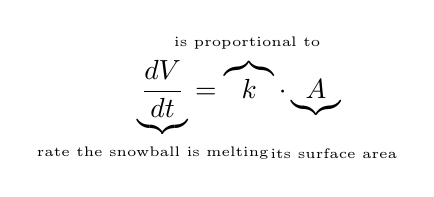
\begin{tikzpicture}
				\node at (0,0) {
					$\underbrace{\frac{dV}{dt}} =  \overbrace{k} \cdot \underbrace{A}$
				};
				\node at (-1.1,-.7) {\tiny{rate the snowball is melting}};
				\node at (.1,.7) {\tiny{is proportional to}};
				\node at (1.2,-.7) {\tiny{its surface area}};
				\end{tikzpicture}
			\end{image}
			We need to compute  $\frac{dV}{dt}$. Since $r$ is a function of $t$, we  differentiate both sides of equation $(1)$. 
			So
			\[
			\frac{dV}{dt} = 4\cdot \pi\cdot r^2 \cdot \frac{dr}{dt}.
			\]
			On the other hand,
			\[
			\frac{dV}{dt} = k\cdot A.
			\]
			Therefore, 
			\[
			4\cdot \pi \cdot r^2 \cdot \frac{dr}{dt} =  k\underbrace{\cdot 4\cdot
				\pi \cdot r^2}_{A} .
			\]
			Now, we \textbf{solve} for $\frac{dr}{dt}$ and obtain that
			\begin{align*}
				\frac{dr}{dt} &=  k.\\
			\end{align*}
			Hence, the radius is changing at a constant rate. Notice, in this example we did not have to evaluate quantities at particular time,  because the unknown rate did not depend on time.
		\end{explanation}
	\end{example}
	
	\section{Right triangles}
	
	\begin{example}
		A road running north to south crosses a road going east to west at the
		point $P$.  Cyclist $A$ is riding north along the first road, and
		cyclist $B$ is riding east along the second road.  At a particular
		time, cyclist $A$ is $3$ kilometers to the north of $P$ and traveling
		at $20$ km/h, while cyclist $B$ is $4$ kilometers to the east of $P$
		and traveling at $15$ km/h.  How fast is the distance between the two
		cyclists changing at that time?
		
		
		\begin{explanation}
			First, we \textbf{introduce the variables} $a$, $b$, and $c$, denoting the distance of cyclist $A$ from the point $P$, the distance of cyclist $B$ from the point $P$, and the distance between the two cyclists, in that order. We \textbf{identify} the given rates $\frac{da}{dt}=20$ km/h, $\frac{db}{dt}=15$ km/h, when $a=3, b=4$  and the unknown rate $\frac{dc}{dt}$, when $a=3, b=4$.
			Now, we \textbf{draw a picture}.
			\begin{image}
				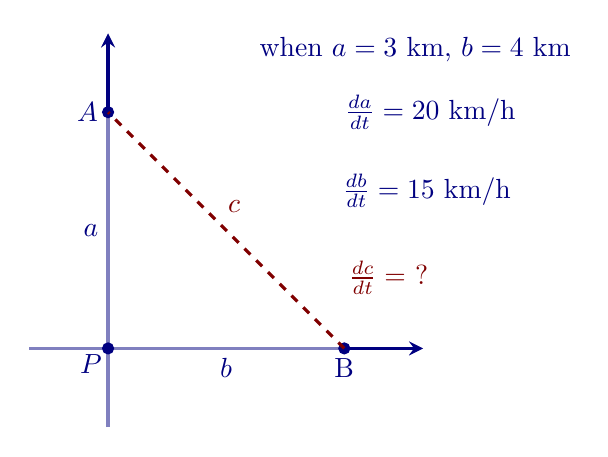
\begin{tikzpicture}
				\draw[->,penColor!50!background, very thick] (-1,0) -- (4,0);
				\draw[->,penColor!50!background, very thick] (0,-1) -- (0,4);
				\draw[->,penColor, very thick] (0,3) -- (0,4);
				\draw[->,penColor, very thick] (3,0) -- (4,0);
				\draw [penColor, fill] (0,0) circle [radius=.07];
				\draw [penColor, fill] (3,0) circle [radius=.07];
				\draw [penColor, fill] (0,3) circle [radius=.07];
				\draw[dashed,penColor2, very thick] (3,0) -- (0,3);
				\node [penColor] at (3.9,3.8) {when $a=3$ km, $b=4$ km};
				\node [penColor,left] at (5.3,3) {$\frac{da}{dt}=20$ km/h};
				\node [penColor, right] at (2.85,2) {$\frac{db}{dt}=15$ km/h  };
				\node [penColor2,left] at (4.19,0.9) {$\frac{dc}{dt}=$ ?};
				
				%\node[penColor,rotate=90,right] at (.5,3) {\scalebox{-2} \Bicycle};
				\node[penColor,right] at (-0.48,-.2) {$P$};
				\node[penColor,left] at (0,1.5) {$a$ };
				\node[penColor,left] at (-.005,3) {$A$ };
				\node[penColor,below] at (1.5,0) {$b$ };
				\node[penColor,below] at (3,0) {B};
				\node[penColor2,above] at (1.6,1.6) {$c$};
				%\node[penColor,right,above] at (3.5,0) {\scalebox{-2}[2] \Bicycle};
				\end{tikzpicture}
			\end{image}
			We \textbf{find equations} relating the variables $a$, $b$, and $c$.  By the Pythagorean Theorem,
			\[
			(1)\hspace{0.2in}c^2=a^2+b^2.
			\] 
			Since  $a$, $b$, and $c$ are functions of time, we \textbf{differentiate} both sides of  the equation with respect to $t$. 
			\[
			(2)\hspace{0.2in}2\cdot c\cdot \frac{dc}{dt}=2\cdot a\cdot \frac{da}{dt}+2\cdot b\cdot \frac{db}{dt}.
			\]
			This equation holds on some time interval, and , in particular, at the instant when $a=3$ and $b=4$. Therefore, at that instant,
			
			\[
			(3)\hspace{0.2in}2\cdot c \cdot \underbrace{\frac{dc}{dt}}_{unknown\hspace{0.015in} rate} =2\cdot 3\cdot \underbrace{20}_ {given\hspace{0.02in} rate}+2\cdot 4  \cdot \underbrace{15}_{given\hspace{0.02in} rate} .
			\]
			
			In order to evaluate $c$, the distance between the cyclists, at the instant when $a=3$ and $b=4$,
			we draw a picture ``taken" at that instant.
			\begin{image}
				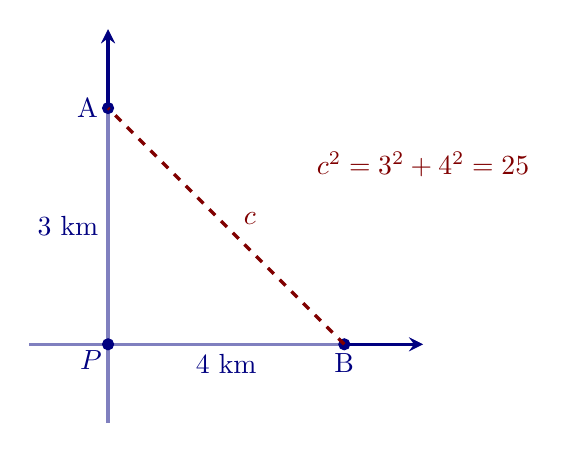
\begin{tikzpicture}
				\draw[->,penColor!50!background, very thick] (-1,0) -- (4,0);
				\draw[->,penColor!50!background, very thick] (0,-1) -- (0,4);
				\draw[->,penColor, very thick] (0,3) -- (0,4);
				\draw[->,penColor, very thick] (3,0) -- (4,0);
				\draw [penColor, fill] (0,0) circle [radius=.07];
				\draw [penColor, fill] (3,0) circle [radius=.07];
				\draw [penColor, fill] (0,3) circle [radius=.07];
				\draw[dashed,penColor2, very thick] (3,0) -- (0,3);
				
				%\node[penColor,rotate=90,right] at (.5,3) {\scalebox{-2} \Bicycle};
				\node[penColor,right] at (-0.48,-.2) {$P$};
				\node[penColor,left] at (-.005,3) { A};
				\node[penColor,left] at (0,1.5) {$3$ km};
				\node[penColor,below] at (1.5,0) {$4$ km};
				\node[penColor,below] at (3,0) {B   };
				\node[penColor2,above] at (1.8,1.4) {$c$};
				\node[penColor2,above] at (4,2) {$c^2=3^2+4^2=25$};
				%\node[penColor,right,above] at (3.5,0) {\scalebox{-2}[2] \Bicycle};
				\end{tikzpicture}
			\end{image}
			By the the Pythagorean Theorem and the picture above, when $a=3$, $b=4$, it follows that
			\[
			c= \answer[given]{5}  km.
			\]
			Now we can  \textbf{evaluate} all the quantities in equation $(3)$ and \textbf{solve} 
			\[
			2\cdot 5 \cdot\frac{dc}{dt} = 2 \cdot 3\cdot 20 + 2 \cdot 4 \cdot 15.
			\]
			We find that $\frac{dc}{dt} = 24$ km/hr at the moment when $a=3$, $b=4$.  \\
			
			
		\end{explanation}
	\end{example}
	
	
	\begin{example}
		A plane is flying at an altitude of $3$ miles directly away from you at $500$ mph 
		.  How fast is the plane's distance from you increasing at
		the moment when the plane is flying over a point on the ground $4$
		miles from you?
		
		
		\begin{explanation}
			First, we \textbf{introduce variables} $p$, the distance the plane has traveled after  it flew right above you, and $s$, the distance between you and the plane. 
			The given rate is $\frac{dp}{dt}=500$ mph and the unknown rate is $\frac{ds}{dt}$, when $p=4$.
			Next, we \textbf{draw a picture}.
			\begin{image}
				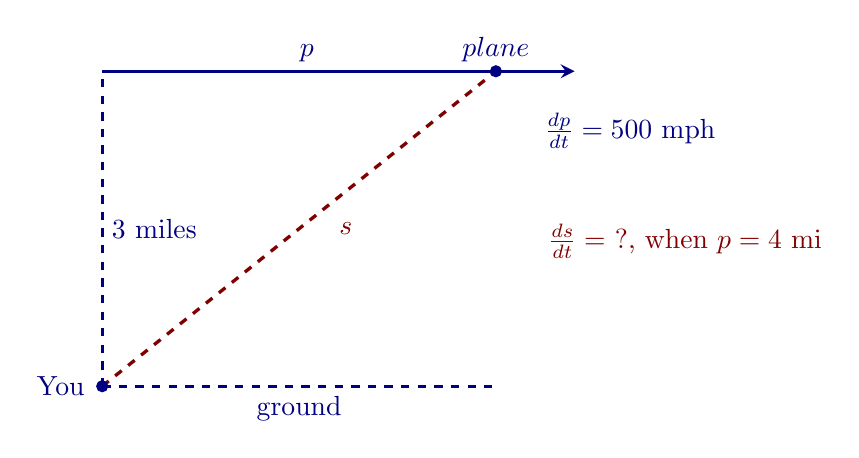
\begin{tikzpicture}
				\draw[penColor2, dashed, very thick] (0,0) -- (5,4);
				%\draw[penColor, dashed, very thick] (0,0) -- (0,4);
				\draw[penColor, dashed, very thick] (0,0) -- (0,4);
				\draw[penColor, dashed, very thick] (0,0) -- (5,0);
				\draw[->,penColor, very thick] (0,4) -- (6,4);
				\draw [penColor, fill] (5,4) circle [radius=.07];
				%\node [left,penColor] at (0,0) {\scalebox{3} \Ladiesroom};
				%\node [right,penColor] at (6,4) {\scalebox{3}{\ding{40}}};
				\node [right,penColor] at (0,2) {$3$ miles};
				\node [above,penColor] at (2.6,4) {$p$ };
				\node [above,penColor] at (5,4) {$plane$ };
				\node [above,penColor] at (6.7,2.9) {$\frac{dp}{dt}=500$ mph};
				\node [above,penColor2] at (7.4,1.5) {$\frac{ds}{dt}=$ ?, when $p=4$ mi};
				\node [below,penColor] at (2.5,0) {ground};
				\node [left,penColor2] at (3.3,2) {$s$ };
				\draw [penColor, fill] (0,0) circle [radius=.07];
				\node [left,penColor] at (-.1,0) {You};
				\end{tikzpicture}
			\end{image}
			Next we \textbf{find equations} relating the variables $p$ and $s$. By the Pythagorean Theorem
			we know that
			\[
			p^2+3^2=s^2.
			\] 
			Since  $p$ and $s$ are functions of time, we now
			\textbf{differentiate} both sides of the equation 
			\[
			2\cdot p\cdot \frac{dp}{dt}  = 2\cdot s \cdot \frac{ds}{dt}.
			\] 
			At the instant when  $p=4$ mi, we get that
			\[
			2\cdot4\cdot\underbrace{ 500}_{given\hspace{0.02in}rate}  = 2\cdot \overbrace{s}^{unknown\hspace{0.02in}value} \cdot \underbrace{\frac{ds}{dt}}_{unknown\hspace{0.02in}rate} .
			\] 
			This implies that $s$ has to be evaluated at time when $p=4$. In order to do that,
			let's draw the picture at the given instant, when $p=4$ mi.
			\begin{image}
				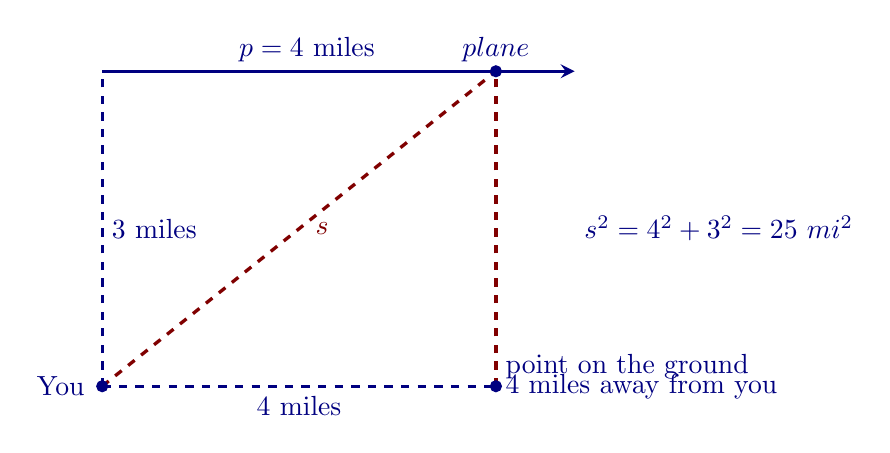
\begin{tikzpicture}
				\draw[penColor2, dashed, very thick] (0,0) -- (5,4);
				\draw[penColor2, dashed, very thick] (5,0) -- (5,4);
				%\draw[penColor, dashed, very thick] (0,0) -- (0,4);
				\draw[penColor, dashed, very thick] (0,0) -- (0,4);
				\draw[penColor, dashed, very thick] (0,0) -- (5,0);
				\draw[->,penColor, very thick] (0,4) -- (6,4);
				\draw [penColor, fill] (5,4) circle [radius=.07];
				\draw [penColor, fill] (5,0) circle [radius=.07];
				%\node [left,penColor] at (0,0) {\scalebox{3} \Ladiesroom};
				%\node [right,penColor] at (6,4) {\scalebox{3}{\ding{40}}};
				\node [right,penColor] at (0,2) {$3$ miles};
				
				\node [right,penColor] at (5,0.25) {point on the ground};
				\node [right,penColor] at (5,0) {4 miles away from you };
				\node [right,penColor] at (6,2) {$s^2=4^2+3^2=25$ $mi^2$};
				\node [above,penColor] at (2.6,4) {$p=4$ miles};
				\node [above,penColor] at (5,4) {$plane$ };
				\node [below,penColor] at (2.5,0) {$4$ miles};
				\node [left,penColor2] at (3,2) {$s$ };
				\draw [penColor, fill] (0,0) circle [radius=.07];
				\node [left,penColor] at (-.1,0) {You};
				\end{tikzpicture}
			\end{image}
			
			
			So, $s=\answer[given]{5}$.  Putting together all the information we get
			\[
			2(4)(500)=2(5)\frac{ds}{dt} .
			\]
			Finally, we \textbf{solve}:  $\frac{ds}{dt}=\answer[given]{400}$ mph, at the moment when $p=4$ miles.
		\end{explanation}
	\end{example}
	
	
	\section{Angular rates}
	
	\author{Nela Lakos}
	\begin{example}
		A plane is flying at an altitude of $3$ miles directly away from you at $500$ mph 
		.  Let  $\theta$ be the \textbf{angle of elevation} of the plane, i.e., the angle between the ground and your line of  sight to the plane.
		How fast is the angle $\theta$  changing at
		the moment when the plane is flying over a point on the ground $4$
		miles from you?
		
		
		\begin{explanation}
			First, we \textbf{introduce a variable} $p$, the distance the plane has traveled after it flew right above you. 
			So, the given rate is $\frac{dp}{dt}=500$ mph and the unknown (related) rate is $\frac{d\theta}{dt}$, at the instant when $p=4$ miles.
			This rate should be measured in rad/s.
			Therefore, we have to convert the units of the given rate, mph, into mi/s:
			$\frac{dp}{dt}=500$mph$=\frac{500}{60\cdot60}$ mi/s. \\
			Next, we \textbf{draw a picture}.
			\begin{image}
				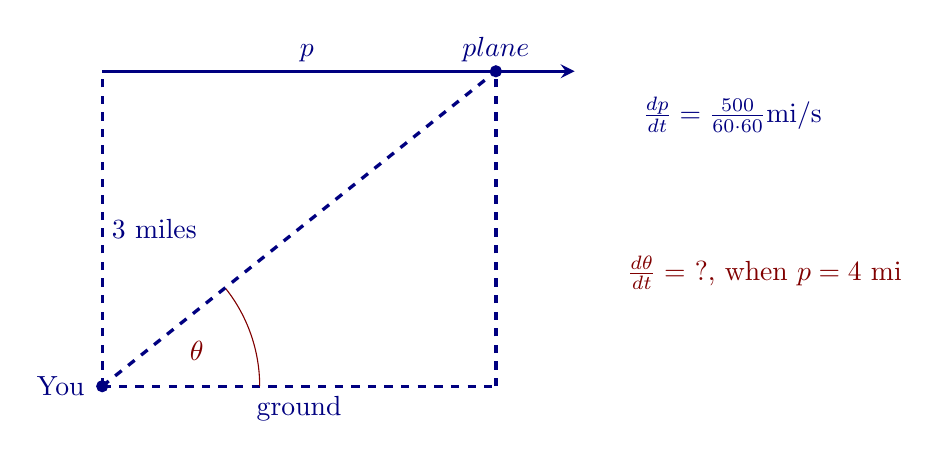
\begin{tikzpicture}
				\draw[penColor, dashed, very thick] (0,0) -- (5,4);
				%\draw[penColor, dashed, very thick] (0,0) -- (0,4);
				\draw[penColor, dashed, very thick] (0,0) -- (0,4);
				\draw[penColor, dashed, very thick] (5,0) -- (5,4);
				\draw[penColor, dashed, very thick] (0,0) -- (5,0);
				\draw[->,penColor, very thick] (0,4) -- (6,4);
				\draw [penColor, fill] (5,4) circle [radius=.07];
				\coordinate (A) at (3.3,2.6);
				\coordinate (B) at (0,0);
				\coordinate (C) at (4,0);
				\tkzMarkAngle[penColor2,size=2cm,thin](C,B,A)
				\node [above,penColor2] at (1.2,0.2) {$\theta$ };
				%\node [left,penColor] at (0,0) {\scalebox{3} \Ladiesroom};
				%\node [right,penColor] at (6,4) {\scalebox{3}{\ding{40}}};
				
				\node [right,penColor] at (0,2) {$3$ miles};
				\node [above,penColor] at (2.6,4) {$p$ };
				\node [above,penColor] at (5,4) {$plane$ };
				\node [above,penColor] at (8,3.1) {$\frac{dp}{dt}=\frac{500}{60\cdot60}$mi/s};
				\node [above,penColor2] at (8.41,1.1) {$\frac{d\theta}{dt}=$ ?, when $p=4$ mi};
				\node [below,penColor] at (2.5,0) {ground};
				\draw [penColor, fill] (0,0) circle [radius=.07];
				\node [left,penColor] at (-.1,0) {You};
				\end{tikzpicture}
			\end{image}
			Now we  \textbf{find an equation} relating variables $p$ and $\theta$.
			From the picture we can see that
			\[
			\tan{\theta}=\frac{3}{p}.
			\] 
			Since  $p$ and $\theta$ are both functions of time, we now
			\textbf{differentiate} both sides of the equation. We write
			\[
			\sec^{2}{\theta}\cdot\frac{d\theta}{dt}  = -\frac{3}{p^2}\cdot \frac{dp}{dt}.
			\] 
			The above equation holds over some interval of time. In particular, it is true when $p=4$. Therefore, when $p=4$,
			\[
			\overbrace{\sec^{2}{\theta}}^{unknown\hspace{0.02in}value}\cdot\underbrace{\frac{d\theta}{dt} }_{unknown\hspace{0.02in}rate} = -\frac{3}{4^2}\cdot\underbrace{ \frac{500}{3600}}_{given\hspace{0.02in}rate}.
			\] 
			This implies that we have to compute the unknown value,  $\sec^{2}{\theta}$, when $p=4$.
			To this end, we  draw and label the picture at the time when $p=4$ mi.
			\begin{image}
				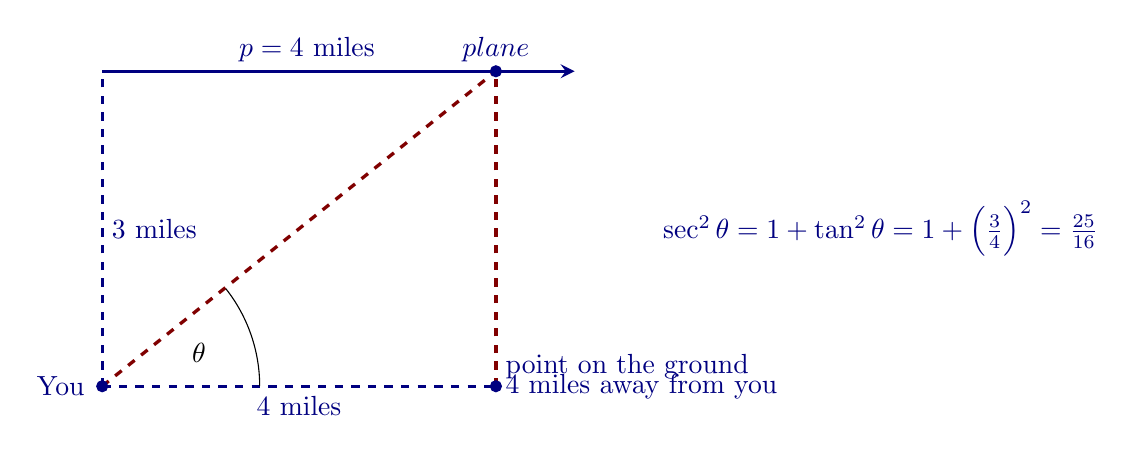
\begin{tikzpicture}
				\draw[penColor2, dashed, very thick] (0,0) -- (5,4);
				\draw[penColor2, dashed, very thick] (5,0) -- (5,4);
				%\draw[penColor, dashed, very thick] (0,0) -- (0,4);
				\draw[penColor, dashed, very thick] (0,0) -- (0,4);
				\draw[penColor, dashed, very thick] (0,0) -- (5,0);
				\draw[->,penColor, very thick] (0,4) -- (6,4);
				\draw [penColor, fill] (5,4) circle [radius=.07];
				\draw [penColor, fill] (5,0) circle [radius=.07];
				\coordinate (A) at (3.3,2.6);
				\coordinate (B) at (0,0);
				\coordinate (C) at (4,0);
				\tkzMarkAngle[size=2cm,thin](C,B,A)
				\tkzLabelAngle[pos = 1.3](C,B,A){$\theta$}
				%\node [left,penColor] at (0,0) {\scalebox{3} \Ladiesroom};
				%\node [right,penColor] at (6,4) {\scalebox{3}{\ding{40}}};
				\node [right,penColor] at (0,2) {$3$ miles};
				\node [right,penColor] at (7,2) {$\sec^{2}{\theta}=1+\tan^{2}{\theta}=1+\Bigl(\frac{3}{4}\Bigr)^2=\frac{25}{16}$ };
				\node [right,penColor] at (5,0.25) {point on the ground};
				\node [right,penColor] at (5,0) {4 miles away from you };
				
				\node [above,penColor] at (2.6,4) {$p=4$ miles};
				\node [above,penColor] at (5,4) {$plane$ };
				\node [below,penColor] at (2.5,0) {$4$ miles};
				\draw [penColor, fill] (0,0) circle [radius=.07];
				\node [left,penColor] at (-.1,0) {You};
				\end{tikzpicture}
			\end{image}
			
			So, at the moment when $p=4$ miles,
			\[
			\sec^2{\theta}=1+\Bigr(\frac{3}{4}\Bigl)^2=\frac{25}{16}.
			\] 
			Now, by substituting all the known values into the equation above, we get
			\[
			\frac{25}{16}\cdot \frac{d\theta}{dt}= -\frac{3}{16}\cdot \frac{500}{3600}.
			\] 
			We \textbf{solve} for $\frac{d\theta}{dt}$, when $p=4$, and get that
			\[
			\frac{d\theta}{dt} = -\frac{1}{60}  rad/s.
			\] 
		\end{explanation}
	\end{example}
	
	\section{Similar triangles}
	
	\begin{example}
		It is night. Someone who is $6$ feet tall is walking away from a
		street light at a rate of $3$ feet per second.  The street light is
		$15$ feet tall.  The person casts a shadow on the ground in front of
		them. How fast is the length of the shadow growing when the person
		is $7$ feet from the street light?
		
		\begin{explanation}
			First, we \textbf{introduce two variables}, $p$, the distance from the person to the lamp, and  $s$, the length of the shadow.
			The given rate is $\frac{dp}{dt}=3$ ft/s and the unknown (related) rate is $\frac{ds}{dt}$ at the moment when $p=7$ feet.
			Next, we \textbf{draw a picture}.
			\begin{image}
				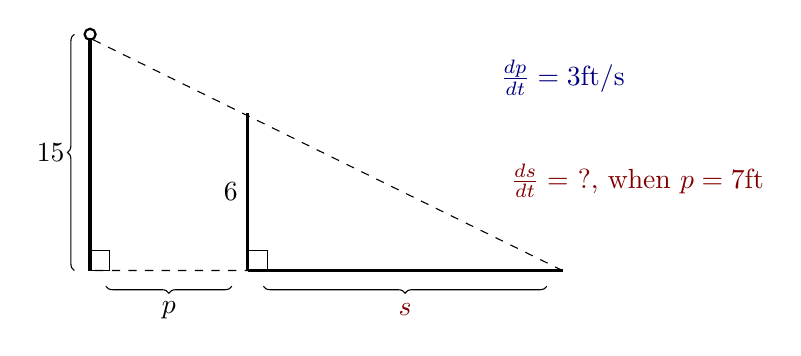
\begin{tikzpicture}
				\coordinate (A) at (6,2);
				\coordinate (B) at (0,4.95);
				\coordinate (C) at (0,2);
				\coordinate (D) at (2,2);
				\coordinate (E) at (2,4);
				\tkzMarkRightAngle(A,C,B)
				\tkzMarkRightAngle(A,D,E)
				\tkzDefMidPoint(A,B) \tkzGetPoint{a}
				\tkzDefMidPoint(A,C) \tkzGetPoint{b}
				\tkzDefMidPoint(D,C) \tkzGetPoint{x}
				\draw[decoration={brace,mirror,raise=.2cm},decorate,thin] (.2,2)--(1.8,2);
				\draw[decoration={brace,mirror,raise=.2cm},decorate,thin] (2.2,2)--(5.8,2);
				\draw[decoration={brace,raise=.2cm},decorate,thin] (0,2)--(0,5);
				\draw[dashed] (A)--(B)--(C)--cycle;
				\draw[very thick] (D)--(E);
				\draw[very thick] (D)--(A);
				\draw[very thick] (B)--(C);
				\node[left] at (2,3) {$6$};
				\node at (1,2-.5) {$p$};
				\node  [penColor2] at (4,2-.5) {$s$};
				\node at (0-.5,3.5) {$15$};
				\node [above,penColor] at (6,4.1) {$\frac{dp}{dt}=3$ft/s};
				\node [above,penColor2] at (6.95,2.8) {$\frac{ds}{dt}=$ ?, when $p=7$ft};
				\draw (0,5)[thick] circle [radius=.07];
				
				\end{tikzpicture}
			\end{image}
			
			Now we \textbf{find equations} that relate the variables $p$ and $s$. We use the fact that we
			have similar triangles to write:
			\begin{align*}
				\frac{s+p}{15} &= \frac{s}{\answer[given]{6}},\\
				6\cdot s + 6 \cdot p &= 15\cdot s,\\
				6\cdot p &=9\cdot s,\\
				2\cdot p &=3 \cdot s. 
			\end{align*}
			Since $p$ and $s$ are both functions of time, we 
			\textbf{differentiate} both sides of the equation above. We  use
			implicit differentiation and write
			\[
			2\cdot \frac{dp}{dt} =3 \cdot \frac{ds}{dt}
			\]
			At this point we \textbf{evaluate} all the quantities at time when $p=7$ ft 
			\[
			2\cdot \cancel{3} = \cancel{3} \cdot \frac{ds}{dt}.
			\]
			Now we \textbf{solve} for  $\frac{ds}{dt}$ and get that
			$\frac{ds}{dt}= \answer[given]{2}$, when $p=7$ ft.
			
			Therefore, the shadow is growing
			at a rate of $2$ ft/s when the person is $7$ ft from the lamp.\\
		\end{explanation}
	\end{example}
	
	
	\begin{example}
		Water is poured into a conical container at the rate of 10
		cm${}^3$/s.  The cone points directly down, and it has a height of
		30 cm and a base radius of 10 cm.  How fast is the water level rising
		when the water is 4 cm deep?
		
		\begin{explanation}
			First, we \textbf{introduce several variables}. Let $V$ be the volume of the water in the container, let $r$ be the radius of the circular surface of the water, and  let $h$ be the depth of the water in the container. The given rate is $\frac{dV}{dt}=10$ $cm^3/s$, and the unknown rate is $\frac{dh}{dt}$, at the moment when $h=4$ cm.
			Now, we \textbf{draw a picture}.
			\begin{image}
				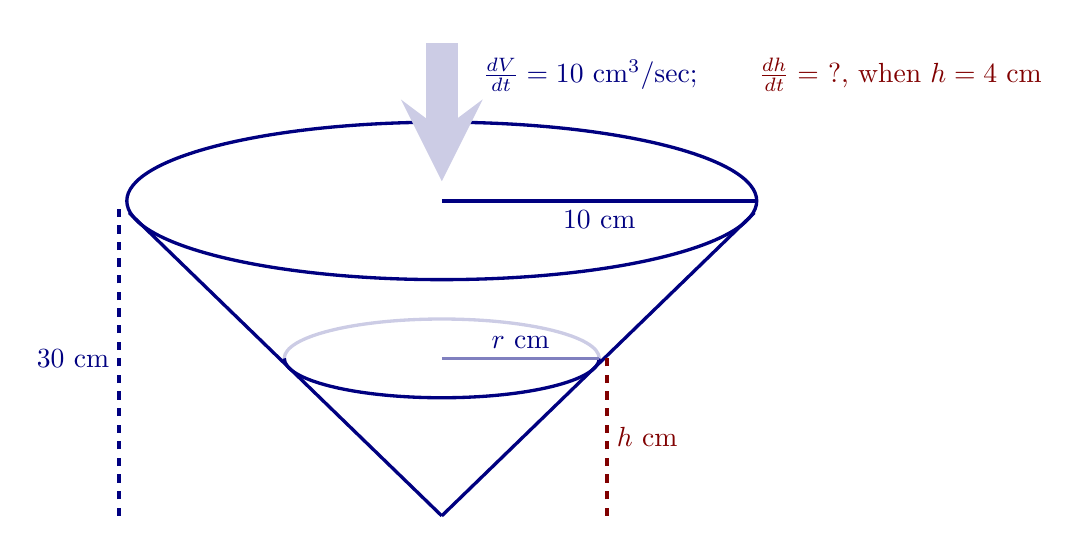
\begin{tikzpicture}
				\draw[penColor,very thick] (0,4) ellipse (4 and 1);
				\draw[very thick,penColor!20!background] (2,2) arc (0:180:2 and .5);% top half of ellipse
				\draw[very thick,penColor] (-2,2) arc (180:360:2 and .5);% bottom half of ellipse
				\draw[penColor, very thick] (3.97,3.85) -- (0,0);
				\draw[penColor, very thick] (-3.97,3.85) -- (0,0);
				\draw[penColor, very thick] (0,4) -- (4,4);
				\draw[penColor!50!background, very thick] (0,2) -- (2,2);
				\draw[->,line width=0.4cm, penColor!20!background] (0,6) -- (0,4.25);
				\draw[dashed, penColor2, very thick] (2.1,0) -- (2.1,2);
				\draw[dashed, penColor, very thick] (-4.1,0) -- (-4.1,4);
				\node[right, penColor] at (.4,5.6) {$\dd[V]{t} = 10$ cm$^3$/sec;};
				\node[right, penColor2] at (3.9,5.6) {$\dd[h]{t} = $ ?, when $h=4$ cm};
				\node[below, penColor] at (2,4) {$10$ cm};
				\node[above, penColor] at (1,2) {$r$ cm};
				\node[right, penColor2] at (2.1,1) {$h$ cm};
				\node[left, penColor] at (-4.1,2) {$30$ cm};
				\end{tikzpicture}
			\end{image}
			Note, no attempt was made to draw this picture to scale, rather we
			want all of the relevant information to be available to the
			mathematician.
			
			Now we \textbf{find equations} that relate all the variables. Notice that water in the container assumes the shape of the container. In this example, the shape is a cone. Therefore, we use the formula for the volume of
			a cone 
			\[
			V = \frac{\pi}{3} r^2 h.
			\]
			Let's draw a cross section of the cone.
			\begin{image}
				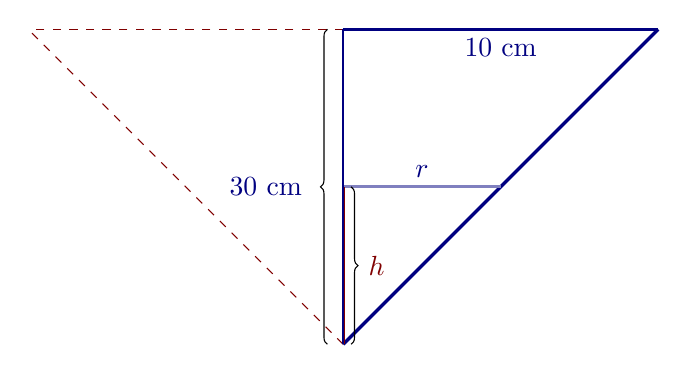
\begin{tikzpicture}
				\draw[penColor, very thick] (4,4) -- (0,0);
				\draw[penColor, very thick] (0,4) -- (4,4);
				\draw[penColor2, thick] (0,2) -- (0,0);
				\draw[penColor!50!background, very thick] (0,2) -- (2,2);
				\draw[dashed, penColor2,  thin] (0,0) -- (-4,4);
				\draw[dashed, penColor2, thin] (0,4) -- (-4,4);
				\draw[ penColor2, very thick] (0,0) -- (0,2);
				\draw[ penColor,thick] (0,0) -- (0,4);
				\draw[decoration={brace,raise=.2cm},decorate,thin] (0,0)--(0,4);
				\draw[decoration={brace, mirror,raise=.1cm},decorate,thin] (0,0)--(0,2);
				\node[below, penColor] at (2,4) {$10$ cm};
				\node[above, penColor] at (1,2) {$r$ };
				\node[right, penColor2] at (0.2,1) {$h$ };
				\node[left, penColor] at (-0.4,2) {$30$ cm};
				\end{tikzpicture}
			\end{image}
			Notice a big right triangle and  a smaller right triangle inside the big one.
			These two right triangles are similar, because their corresponding angles are equal.
			Since the ratios of corresponding sides in similar triangles are equal, we get
			\[
			\frac{r}{h}=\frac{10}{30} \qquad\text{so}\qquad r=\frac{h}{\answer[given]{3} }.
			\]  
			At this point we could \textbf{differentiate} both sides of each equation, but we can take a simpler approach
			by combining these two equations and expressing $V$ in terms of $h$.
			
			QUESTION: Why is it more convenient to express $V$ in terms of $h$ than in terms of $r$?
			
			Therefore,
			\[
			V = \frac{\pi}{3}\overbrace{ \Bigl(\frac{h}{3}\Bigr)^2}^{r^2} h,
			\]
			and
			\[
			V = \frac{\pi}{27} \cdot h^3.
			\]
			Now, we \textbf{differentiate} with respect to $t$.
			\[
			\dd[V]{t} = \frac{\pi}{27} \cdot 3\cdot h^2\cdot \frac{dh}{dt}.
			\]
			This  equation holds over some time interval. In particular, the equation is true at time when $h=4$ cm. 
			Now we \textbf{evaluate} all the quantities at that time.
			\[
			10 = \frac{\pi}{27} \cdot 3\cdot 4^2\cdot \frac{dh}{dt}.
			\]
			So, at the instant when the water in the container is $4$ cm deep, the water level is rising at the rate of $\frac{45}{8\pi}$ cm/s.
		\end{explanation}
	\end{example}
\end{document}



